\RequirePackage[abort, l2tabu, orthodox]{nag}
\documentclass[pageno]{jpaper}

% standard LaTeX packages that do not interfere with hyperref
\usepackage{alltt}
\usepackage{amssymb}
\usepackage{booktabs}
\usepackage{caption}
\usepackage[draft]{fixme}
\usepackage{epstopdf}
\usepackage{flushend}
\usepackage{graphicx}
\usepackage[final]{listings}
\usepackage[sort&compress]{natbib}
\usepackage{tikz}
\usepackage[normalem]{ulem}
\usepackage{xspace}

% font selection
\usepackage{courier}
\usepackage{helvet}
\usepackage{mathptmx}
\usepackage{microtype}
\usepackage[mathscr]{euscript}

% hyperref itself
\usepackage{hyperref}

% standard packages that must be loaded after hyperref
\usepackage{bookmark}
\usepackage{verbatim} 

% should be loaded after listings and subfig
\usepackage{cleveref}
\usepackage{multirow}
\usepackage{xfrac}

% custom packages for this paper
 
%\DeclareCaptionType{copyrightbox}

\renewcommand{\cite}[1]{%
  \PackageError{natbib}{%
    The \string\cite\space{} command is ambiguous; use
    \string\citet\space{} or \string\citep\space{} instead}{}}

\renewcommand{\autoref}[1]{%
  \PackageError{cleveref}{%
    Do not use \string\autoref.  Use \string\cref instead, or use
    \string\crefrange for ranges of referenced items}}

\renewcommand{\hline}[1]{%
  \PackageError{booktabs}{%
    Do not use \string\hline.  Use \string\toprule, \string\midrule,
    or \string\bottomrule\space instead depending on where in the
    table the line appears}}

\newcommand{\email}[1]{\href{mailto:#1@cs.cmu.edu}{#1}}

% cleveref configuration
\crefname{figure}{Figure}{Figures}
\crefname{section}{Section}{Sections}
\crefname{table}{Table}{Tables}

\hyphenation{test-case}

% lst configuration
\lstdefinelanguage{example}{%
  morekeywords={xyz},
}

\lstset{
  basicstyle=\sffamily,
  columns=fullflexible,
  numbersep=5pt,
  numberstyle=\scriptsize,
  showstringspaces=false,
  language=example,
  escapeinside={/*@}{@*/},
  belowcaptionskip=1\baselineskip,
  language=C,
  showstringspaces=false,
  keywordstyle=\bfseries,
  commentstyle=\itshape,
}


\urlstyle{sf}

\pdfpagewidth=8.5in
\pdfpageheight=11in


% Custom commands
\newcommand{\Tool}{\textsc{XYZ}\xspace}

%\sloppy
% start doc
\begin{document}

\title{Hardware Transactional Memory Support for Multi-Key Transactions\\
\large{CS 15-712 Project Midway Report}}

\author{Joy Arulraj \hspace{0.1 in} Jesse Dunietz \hspace{0.1 in} Thomas Marshall\\ 
{\{\email{jarulraj}, \email{jdunietz}, \email{twmarsha}\}}}

\date{}
\maketitle


\begin{abstract}
  Hardware transactional memory (HTM) has long been theorized to offer many
  benefits for concurrent programming, but a dearth of implementations has
  inhibited real-world tests. Recent Intel processors have introduced support
  for HTM in the form of transaction synchronization instruction set
  extensions. These extensions provide two software interfaces to define
  transaction regions: a flexible interface which allows the programmer to
  specify a fallback path to handle transaction failures (Restricted
  Transactional Memory) and another backward-compatible interface that is less
  customisable (Hardware Lock Elision). We applied these new hardware primitives
  to control concurrency in transactions on an in-memory key-value store, and
  compared their performance against traditional pessimistic concurrency control
  schemes \footnote{Source code of the project is available at : 
  \url{https://github.com/jarulraj/CMU-OS/tree/master/code}}.  
  We tested multiple-key transactions with both static and dynamic
  read/write sets. Our results indicate that, at least in this setting, HTM
  performance is essentially comparable with similarly structured lock-based
  schemes. HTM thus appears unlikely to offer significant performance benefits, 
  though it may still ease the burden on programmers.
\end{abstract}

\section{Introduction} \label{sec:intro}

Transactional memory (TM) is a mechanism to provide
fine-grained read/write access to multiple memory words in a lock-free manner
\citep{Herlihy93}. Several implementations of TM have been realized in hardware
and software. For instance, the load linked/store conditional primitive available
in modern processors is a special form of TM, where access is regulated to only
one memory word. Hardware implementations generally rely on extensions to the
cache-coherence protocol. Software implementations, on the other hand, provide
transactional interfaces by using basic hardware primitives like atomic compare and
swap (CAS).

In recent Intel Haswell processors, transactional memory support has been added
in the form of instruction set extensions known as Transaction Synchronization
Extensions (TSX). TSX supports two interfaces \citep{tsx-intro}: \\

\begin{itemize} 
\item \textbf{Hardware Lock Elision (HLE)} \\ This is a backward
compatible extension which allows specification of transaction regions using
\textrm{XACQUIRE} and \textrm{XRELEASE} prefixes. It is compatible with the lock-based programming
model. In HLE, when the transaction execution fails, the TM implementation
simply reverts to normal lock semantics during re-execution. \\ 

\item \textbf{Restricted Transactional Memory (RTM)} \\ This is a more
flexible extension, albeit not a backward compatible one, which allows specification of
transactions using \textrm{XBEGIN, XEND and XABORT} instructions. It allows the
programmer to specify the fallback path when the transaction fails.  \\ 
\end{itemize}

These hardware primitives can be used to implement concurrency control 
required for synchronizing accesses to data structures. In this project,
we plan to focus specifically on \textit{multi-key transactions} on a
\textit{key-value store}. In \Cref{sec:tm},
we describe the problem of synchronizing multi-key transactions on a 
key-value store using hardware TM support.
We then present the traditional pessimistic concurrency control protocols 
we plan to use for comparison in \Cref{sec:pessimistic}. Finally, we
define the goals of this project and our plan to split the workload
in \Cref{sec:plan}.

\section{Optimistic Concurrency Control in Haswell} \label{sec:tm}

A simple mechanism that can be used to provide atomicity and isolation is
coarse-grained locks. This allows at least a limited amount of safe concurrency.
However, this is a pessimistic concurrency control protocol that targets
\textit{high-contention} workloads. Read accesses also need to incur the locking overhead
in this scheme.

For low-contention workloads (e.g, read-dominant workloads), an optimistic
concurrency control scheme generally provides better performance, as
transactions can be mostly executed in parallel, and only the few that conflict
will need to be aborted or retried. (Optimistic concurrency control mechanisms
generally still rely on locking to validate and commit speculatively executed
changes, but this critical section is relatively small.) This allows
non-conflicting accesses to avoid the overhead of locking, providing a
significant boost in throughput.

Originally proposed in the context of database transaction managers, OCC schemes
have also been applied to concurrent programming, in the form of transactional
memory. Such schemes expose very little of the concurrency control protocol to
the user. Instead of requiring the programmer to maintain complex locking code,
all of complexity of concurrency control is pushed lower in the programming
stack: to the language runtime layer (in the case of software transactional
memory schemes) or to the hardware layer (in the case of HTM schemes). The
programmer is presented only with the higher-level abstraction of
transactions. Transactional memory thus provides the additional benefit of
greatly simplifying concurrent programming.

Intel's Haswell processor provides a transactional memory abstraction at the
hardware level. Transactions are executed within a core's own L1 cache, and the
cache-coherence protocol is extended to check at commit time whether other cores
have committed conflicting writes. This implementation allows non-conflicting
transactions to elide locks entirely, serializing only conflicting transactions.

The Haswell processors implement HTM in the form of instruction set extensions
known as Transaction Synchronization Extensions (TSX). TSX supports two
interfaces \citep{tsx-intro}: \\

\begin{itemize} 
\item \textbf{Hardware Lock Elision (HLE):} \\ This is a backwards-compatible
  extension which allows specifying transaction regions via \texttt{XACQUIRE}
  and \texttt{XRELEASE} instruction prefixes. These prefixes are added to a set
  of existing atomic load/store instructions which are typically used to
  read/write locks. When the \texttt{XACQUIRE} prefix is included, the locking
  code is speculatively elided, and the transaction is checked for conflicts
  when the \texttt{XRELEASE} prefix next appears. If conflicts have occurred,
  transaction execution fails, and the TM implementation simply reverts to
  normal lock semantics: the transaction is re-executed, but this time using the
  normal load/store instructions. HLE is thus fully compatible with the
  conventional, lock-based programming model. \\
\item \textbf{Restricted Transactional Memory (RTM):} \\ This is a more flexible
  extension, albeit not a backward compatible one, which allows specification of
  transactions using new \texttt{XBEGIN}, \texttt{XEND}, and \texttt{XABORT}
  instructions. It allows the programmer to specify the fallback path for
  transaction failures. An example of a group sum operation using RTM interface
  is shown in \Cref{fig:rtm}.\\
\end{itemize}

\lstset{basicstyle=\ttfamily\fontsize{9}{10}\selectfont,
morekeywords={if,else,end}, numbers=left} \begin{figure}
    \parbox[t]{0.45\textwidth}{\lstinputlisting{figure/rtm.c}} \caption{Group
        sum operation using RTM interface. A mutex is obtained in fallback path
to avoid data race with the normal transaction execution path.} \label{fig:rtm}
\end{figure}

We evaluated both interfaces in this project. We implemented two different 
RTM schemes and one HLE scheme.
The \textit{simple RTM manager} nests the entire transaction execution within the RTM
instructions \texttt{XBEGIN} and \texttt{XEND} and grabs a mutex in the fallback path.
The more sophisticated \textit{RTM manager} only protects accesses to the lock table 
using the RTM instructions and the transaction execution itself is not in the critical 
path. We designed this scheme to perform well especially for large multi-key 
transactions.  
The \textit{HLE manager} is, by design, similar to the sophisticated RTM manager, except 
that it's fallback path involves execution of instructions while ignoring 
the \texttt{XACQUIRE} and \texttt{XRELEASE} prefixes.

When the read/write sets are static (known a priori), we prevent deadlocks in our
fine-grained schemes by enforcing an ordering in which a transaction may request 
locks. For dynamic read/write sets, we observed that using a simple coarse-grained 
lock delivered performance comparable to a more sophisticated fine-grained 
locking scheme with deadlock detection. We therefore use a coarse-grained locking
scheme in all the hardware-based concurrency control managers for handling
dynamic read/write sets effectively. This is a significant engineering benefit that 
we believe exemplifies the benefits of using HTM.  \\

\section{Pessimistic Concurrency Control} \label{sec:pessimistic}

In order to have a baseline against which to compare the performance of HTM, we
will be implementing two different forms of traditional, software based
pessimistic concurrency control using locks - a lock manager and spin locks.

\subsection{Lock Manager}

Traditional locking schemes make use of a lock manager, which arbitrates access
to record in the key-value store by granting locks to requesting transactions on
a per key-value pair basis. A lock manager consists of a lock table hashed on
keys. Each lock record contains a mode, either read, write, or free, and a list
of transactions waiting to acquire the lock. A transaction may only access a
given key-value pair once it has requested and been granted the appropriate
lock, preventing conflicts.

When a process requests a lock, the lock manager grants the request if it is
compatible with the lock's mode, where writes are incompatible with reads and
other writes. This is because only writes can cause conflicts - any number of
transactions can execute concurrent reads without affecting each other. When the
transaction currently holding the lock releases it, the lock manager grants the
lock to the transaction at the head of the waiting queue.

We will prevent deadlocks by enforcing an ordering in which a transaction may
request locks, ensuring that no circular dependencies between transactions
waiting on locks may occur. This works well under our assumption that the read
and write sets of transactions are static, but can be difficult if the read and
write sets cannot always be known at the start of the transactions.\\

\subsection{Spin Locks}

In a spin lock scheme, each key-value pair has an associated memory word
representing its lock. Locks are acquired using an atomic test-and-set
primitive. If a transaction attempts a test-and-set but it fails because the
lock is already held, the transaction "spins", or repeatedly attempts to grab
the lock until it eventually succeeds. As with the lock manager, we will
implement deadlock prevention by enforcing an order in which locks must be
obtained.

By avoiding the extra work of going through the manager, spin locks can
potentially be faster. However, the obvious disadvantage of spin locks is that
they require busy waiting - when a transaction spins while waiting for a lock,
it is using CPU time without really doing any useful work. This is primarily a
problem in systems with high contention, where it is likely that multiple
transactions will want to access the same key-value pair at the same time. Prior
work \citep{tran2010} has demonstrated using simulation that TM peforms well
under low contection workloads and spinlocks work well under high contention
workloads. We plan to evaluate whether this observation is valid in real world
HTM implementation.
%Time required to access a given number of objects using different concurrency
%control protocols, based on their simulation, is shown in \Cref{fig:overhead}. 

% jarulraj: Removed figure for now -- not sure if we need to show it in proposal

%\begin{figure}[h!] \centering
%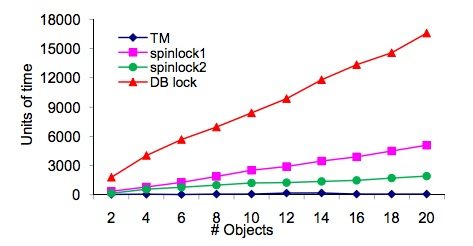
\includegraphics[width=0.45\textwidth]{figure/overhead.jpg} \caption{Overhead
%of different concurrency control protocols under low contention workloads
%\citep{tran2010}.} \label{fig:overhead} \end{figure}

\section{Project Plan} \label{sec:plan}

Broadly speaking, we plan to:
\begin{itemize}
\item implement two different TSX-based concurrency control schemes for a simple key-value store
\item evaluate the performance of that concurrency control scheme under different workloads
\end{itemize}
The goals of the project are as follows:
\begin{itemize}
\item \textbf{75\% goal:} Implement concurrency control for a key-value store with both HLE and RTM, and compare the performance of these two schemes against each other.
\item \textbf{100\% goal:} Additionally, compare the above approaches with traditional pessimistic concurrency control schemes, specifically spin-locks and a basic lock manager. This will demonstrate the advantages of the hardware-based approach for this task, or else show that this task is not one where the hardware-based approach helps.
\item \textbf{125\% goal:} Additionally, implement a software-based (i.e., timestamp-based) OCC scheme and compare it against the above approaches. This will serve as a basic check that it is in fact the hardware that is the cause of any differences in performance, not just the optimistic approach to concurrency.
\end{itemize}

\subsection{Resources Required}
The only resource absolutely necessary for this project is access to a machine with a Haswell processor. Dong has granted us access to a CMU-owned machine.

It would be useful, though not essential, to have access to the existing codebase that has been used by Professor Andersen's lab to run similar HTM experiments in the past. In particular, it would be helpful to have access to the key-value store implementation used in the lab's in-progress study. We are expecting that Dong will be able to give us access to this, as well.

\subsection{Experiments}
Our experiments are inspired by those reported in \citep{tran2010}. We will restrict ourselves to a small, fixed number of key-value store entries. In each experiment, we will measure the time it takes to run a randomly generated workload of datastore operations, given a particular CC scheme. Each workload will simply consist of looking up some set of keys and trivially modifying their values (e.g., incrementing). Specifically, we will run the following experiments for each type of CC mechanism:
\begin{enumerate}
\item With several fixed sizes for read/write sets and numbers of threads, vary the contention level between operations on different threads. This will allow us to determine how each of the CC mechanisms scales with respect to contention.
\item With several different fixed contention levels and numbers of threads, vary the size of the read/write sets. This will allow us to determine how each of the CC mechanisms scales with respect to the read/write set. (For HTM, this may be a very important factor, since transactions abort based on conflicts anywhere in the read/write set.)
\item With several different fixed contention levels and read/write set sizes, vary the number of threads running. This will allow us to determine how much benefit each mechanism is able to benefit from adding more parallelism.
\end{enumerate}

\subsection{Work Plan}
The required steps for executing this project are as follows:
\begin{enumerate}
\item Familiarize ourselves with an existing basic key-value store system, such as that built by Professor Andersen's group, or (if that turns out to be impractical) implement our own. If we end up choosing the latter approach, we can minimize implementation effort by keeping the data structures very simple -- just 1-2 hash tables, one for the data and one for locks or to group data entries larger than a cache line (if applicable).
\item Design the structure of the transaction manager to support multiple CC mechanisms.
\item Using the Haswell TSX APIs, implement a transaction manager that optimistically attempts to execute a transaction, and retries according to either an HLE strategy or a custom RTM-specified strategy.
\item Write a system to generate test workloads with different amounts of contention. It should also allow specifying thread assignments if necessary.
\item Run the experiments for the two HTM approaches. Some tweaking will be necessary to find the most informative thread numbers, read/write set sizes, and contention levels.
\item Implement spin-locks and a lock manager.
\item Rerun the experiments for the pessimistic concurrency control approaches.
\item Implement software-based OCC.
\item Rerun the experiments for OCC.
\item Collate/visualize data and write up report.
\end{enumerate}

All of us will work together on items 1 and 2. Two of us (jdunietz and jarulraj) will collaborate (via pair programming) to implement the TSX-based transaction manager. In parallel, twmarsha will implement the workload generator using an agreed-upon interface. jarulraj and twmarsha will each run preliminary versions of one experiment for item 5, and jdunietz will use their results to run the final experiments and collate/visualize the data. twmarsha will implement a lock manager, jarulraj will implement spin-locks, and jdunietz will implement OCC.

\section{Performance Evaluation} \label{sec:eval}
We first present the experimental setup we used to evaluate both software- and hardware-based concurrency control schemes. We then present the experiments themselves and their results.

\subsection{Experimental Setup}
The architecture of our test program is extremely simple. The tester runs in a
single process, spawning multiple threads within that process' address
space. This eliminates the need for any inter-process communication, which could
confound experimental results. Each thread runs a workload generator, which
generates transactions consisting of fixed-size sequences of reads and
updates. (For the sake of simplicity, we populate the hashtable with values
prior to running the experiments, and allow only read and update operations
during transactions.)

All workload generators pass their transactions to a single transaction manager
(in an unsynchronized fashion). The transaction manager is responsible for
executing the transactions on the underlying hashtable, providing concurrency
control between transactions. Each concurrency control scheme is implemented as
a specialization of the transaction manager interface.

The underlying hashtable is a simple, linear-chaining implementation, ported to
C++ from an open-source C implementation we found online. The simplicity of this
implementation allowed us to ensure that there were no surprising memory
management operations going on behind the scenes.

All tests were performed on a recent Haswell box with support for hardware
transactional memory. All data reflects an average over 3 1-second runs, and
performance is measured in millions of hashtable operations per second.

Possible parameters that we could have varied included: the distribution of keys
accessed, number of workload threads, number of operations per transaction,
number of distinct keys accessed per transaction, length of values being stored,
ratio of reads to writes, whether the read/write sets are static or dynamic, the
total number of keys present in the hashtable, and the number of aborts to allow
before reverting to the fallback path in the hardware based schemes. Because
trying every possible combination of these parameters would result in an
overwhelming amount of data, we kept several of them constant throughout the
tests:
\begin{itemize}
\item All tests use a Zipfian distribution for key accesses, which we believe is
  representative of many real world-workloads.
\item All values are random strings of length 4.
\item The ratio of reads to writes is 1:1. (This is not fully representative of
  real workloads, but this parameter was found to have little impact on
  performance numbers).
\item The hashtable contains 16384 keys, which we estimated to be appropriate
  for the cache size of the machine we were running the experiments on.
\item The maximum allowed retries after abort is tuned to what we found to be
  the optimal value on a per-scheme basis.
\end{itemize}

\subsection{Varying Contention}

One of the most important differences between the schemes that we compared is
their performance in the face of varying levels of contention. In order to
measure this, we implemented two different workload parameters related to
contention. The \textit{transaction size} parameter determines the amount of
work each transaction does, measured by the number of hashtable operations each
transaction performs.  The \textit{keys per transaction} parameter determines
the number of distinct keys that each tranaction acts on: each transaction draws
this many keys from the key distribution, then cycles through those keys for the
transaction operations. If a transaction touches a larger number of keys, it
will likely generate a higher degree of contention, as its key set will overlap
more with those of other transactions. In combination, these parameters allow us
to observe the effect of increasing contention in the presence of large or small
transactions.

\begin{figure}[h!]
  \centering
  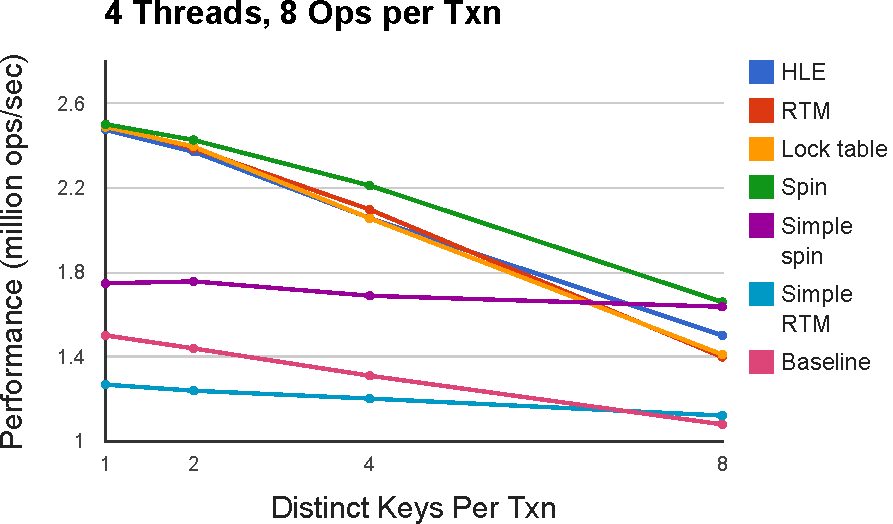
\includegraphics[scale=0.575]{figure/small_txns.pdf}
  \caption{Effect on different schemes of varying contention, using small
    transactions.}
  \label{fig:small_txns} 
\end{figure}

The results of varying contention when using small transaction sizes are shown
in \Cref{fig:small_txns}. For this experiment, we used transactions that
performed 8 operations on the hashtable, while varying the number of distinct
keys that each transaction touches from 1 to 8. The data reflects 4 running
threads, which we found to be the ``sweet spot'' for generating a large enough
workload to saturate the CPU without overwhelming it. The baseline is an
exception: it was run single-threaded and without any concurrency control.

As the graph shows, the baseline implementation is relatively unaffected by the
increase in contention -- it is single threaded, so it never has to stop
transactions to wait for another to complete. The slight drop in performance is
due to the increased amount of time that it takes to generate transactions with
a large number of keys.

The simple spin lock implementation is similarly unaffected by increased
contention, because it grabs a single lock for the entire table for each
transaction regardless of the keys in the transaction. This scheme achieves a
higher throughput than the baseline implementation, and is also less affected by
increases in contention. This is because per-transaction overheads, such as
the generation of the keys each transaction will touch, are not performed in the
lock's critical section, allowing for a very small degree of parallelism that
the baseline implementation does not have.

The worst performace is achieved by the simple RTM scheme, which aborts
essentially every transaction due its na\"{\i}ve use of hardware transactional
memory.  As a result, it falls back to using a single lock to protect the entire
table on every transaction. This leads to performance that does not degrade with
increased contention -- exactly like the simple spin lock's, but with
significantly lower throughput due to time spent aborting and retrying
transactions.

All of the other schemes are fine-grained to increase concurrency, and as a
result their performance degrades as contention is increased.

The hardware schemes do not perform any better than the software schemes. We
believe that this is because there are two competing effects at work. On the one
hand, locks are sometimes successfully elided and transactions are able to
complete successfully without interference. In this case, the HTM schemes are
faster than the software schemes, which never elide locks.  However, if a
conflict causes HTM to abort, it must re-execute the transaction, making it
slower than the software methods. When the maximum number of aborts before
locking the entire table is configured optimally for the hardware schemes, these
factors roughly cancel each other out. This also accounts for the greater drop
in performance of the hardware-based schemes as contention increases, since
greater contention leads to more aborts.

A final takeaway from this graph is that the performance of fine-grained spin
locks is better than that of the fine-grained lock table under high contention,
presumably because spin locks impose less overhead. In particular, spin locks do
not force the many context switches that a lock table causes by sleeping and
waking threads for each conflict.

\begin{figure}[h!]
  \centering
  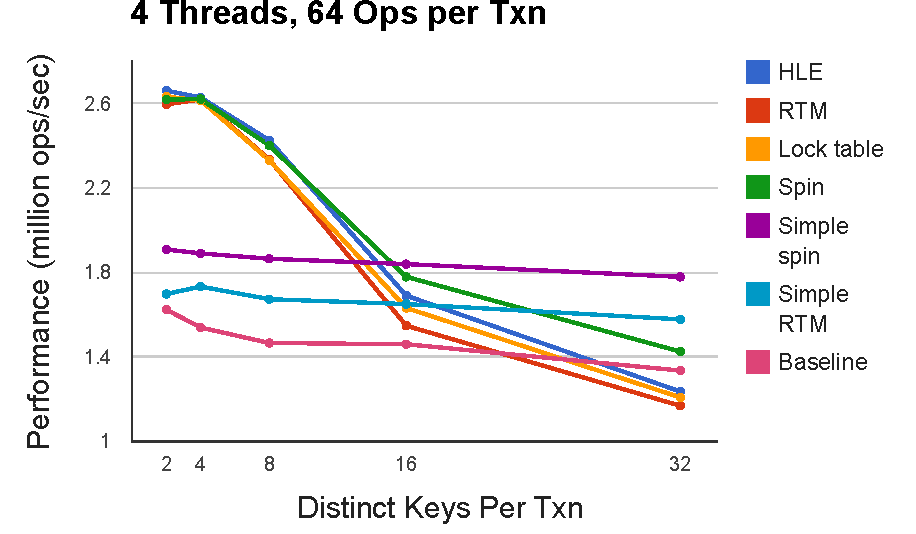
\includegraphics[scale=0.575]{figure/large_txns.pdf}
  \caption{Effect on different schemes of varying contention, using large
    transactions.}
  \label{fig:large_txns} 
\end{figure}

We also wanted to measure the effects of increased contention while using a
large transaction size. The results of this experiment are reflected in
\Cref{fig:large_txns}. For this experiment, we used transactions that performed
64 hashtable operations, and varied the number of distinct keys in each
transaction from 2 to 32. As with the small transactions, results reflect
running with 4 threads, except for the baseline which uses one thread.

As expected, the shape of the different schemes' performance follows the same
pattern as for the experiment with small transactions. The peak throughput here
is somewhat higher -- over 2.6 million, versus about 2.5 million for small
transactions. This is because each transaction performs more work, so there is
less of a slowdown from per-transaction overheads such as passing the
transaction to the transaction manager. Despite the significant increase in
transaction size, this effect is small because most of the per-transaction
overhead, such as generating keys for the transaction, increases with more
operations per transaction.

It is also noteworthy that the performance of the fine-grained schemes degrades
much more dramatically here than in the small transactions experiment. This is
partially due to a much longer per-transaction critical section, which results
in longer lock waits in the lock-based schemes and more aborts in the
hardware-based schemes. Another cause is the fact that this experiment achieves
much higher contention than the small-transaction test. Our hashtable contains
only $2^{14}$ keys, and the Zipfian distribution of key accesses produces a
large number of accesses to a small number of ``hot'' keys. With up to 4
transactions attempting to run simultaneously, if each transaction touches 32
distinct keys, the probability of each transaction conflicting with another is
extremely high.

In fact, as the graph demonstrates, when the contention becomes high enough it
is actually more efficient to use a simple spin lock than one of the more
sophisticated schemes. This is because fine-grained locking adds a large amount
of overhead, and in the case of very high contention adds little to the
potential concurrency of the system.

\subsection{Varying Threads}

Another effect that we wished to study is the performance of the different
schemes under heavier and lighter workloads. We determined the intensity of the
workload by varying the number of threads concurrently accessing the hash
table. (The baseline was again run for a single thread, this time with its
results averaged over 9 runs.)

\begin{figure}[h!]
  \centering
  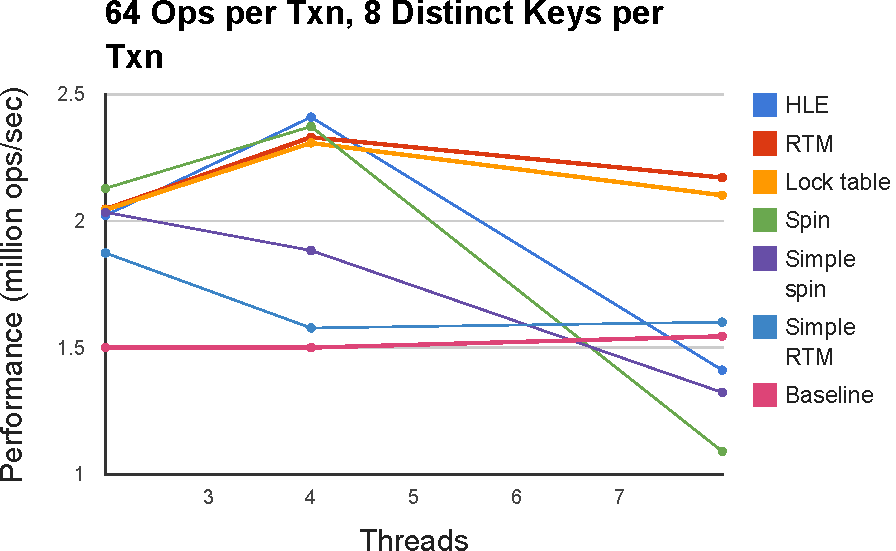
\includegraphics[scale=0.575]{figure/threads.pdf}
  \caption{Effect on different schemes of varying the number of threads.}
  \label{fig:threads} 
\end{figure}

The results of this experiment as shown in \Cref{fig:threads}. In this
experiment, we varied the number of threads from 2 to 8. We used large
transactions (64 operations each) and a moderate level of contention, with each
transaction working on 8 distinct keys.

As expected, most of the schemes follow the pattern of initially increasing in
performace, peaking at around 4 threads, and then declining with increasing
threads. This is because a very small number of threads does not take advantage
of all of the potential parallelism, resulting in lower throughput, whereas a
very large number of threads results in too much contention and degrades
performance as a result.

When we varied contention for a single workload (see \Cref{fig:large_txns}), the
fine-grained spin lock implementation performed better than the lock table
implementation. Increasing the workload size gives the opposite result. This
results from contention for CPU resources: spin locks suffer because they impose
a constant load on the CPU, whereas the lock table simply puts threads to sleep
while they are waiting on a lock to become free. This allows the lock table to
handle a high number of threads more gracefully.

It is also noteworthy that RTM's performance is similar to that of the lock
table's, whereas HLE's performance more closely matches that of the fine-grained
spin locks.  This is because the fallback path for HLE is to grab a 
spin lock, whereas the fallback path for RTM was configured to use a 
mutex, like the locks in the lock table.

The other schemes do not follow this same pattern of increasing then decreasing
performance. In particular, the simple spin lock scheme does not show any
increase in performace, as it only allows a single transaction to execute at a
time regardless of the number of threads.

\subsection{Dynamic Read/Write Sets}

The final experiment that we ran measured the effects of dynamic read/write sets
on the different concurrency control methods. This is significant because it
leads to the possibility of deadlock, which we avoided in the previous
experiment by enforcing an ordering in which the locks would be grabbed by the
fine-grained schemes.

For this experiment, we reused the parameters from the second experiment:
large transactions of 64 operations, 4 running threads, and varying 
contention by increasing the number of distinct keys for each transaction 
from 2 to 32.

\begin{figure}[h!]
  \centering
  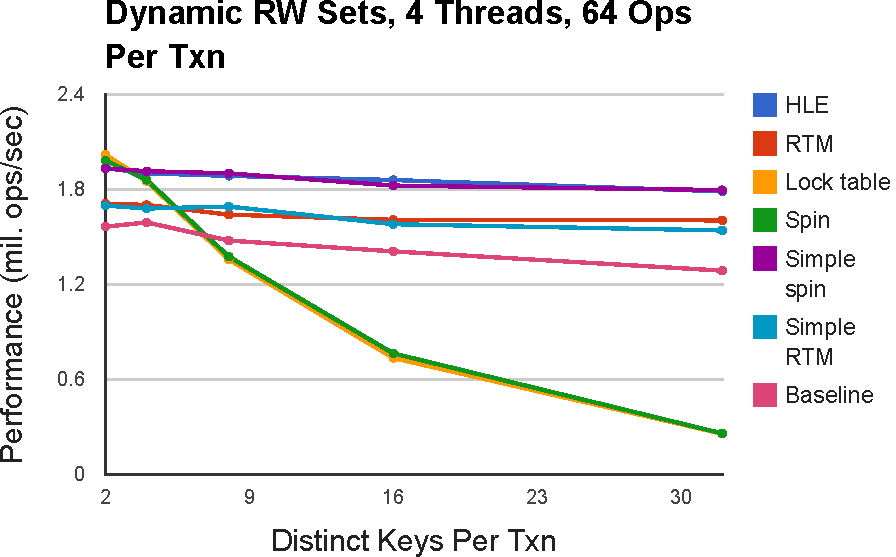
\includegraphics[scale=0.575]{figure/dynamic.pdf}
  \caption{Effect of dynamic read/write sets.}
  \label{fig:dynamic} 
\end{figure}

As \Cref{fig:dynamic} reflects, dynamic read/write sets have a dramatic impact
on the performance of the software-based schemes, resulting from the possibility
of deadlocks. We deal with deadlocks by timing out transactions that have been
waiting on a lock too long and aborting them. As contention increases, the
number of aborts becomes very high, dramatically reducing the throughput by more
than a factor of 2.

In contrast, the performance of the hardware-based schemes is unaffected by 
the dynamic read/write sets. This is because the only time these schemes 
actually grab a lock is in the fallback path, in which case there is only a 
single lock for the entire table and therefore no possibility of deadlock.

Admittedly, our deadlock prevention method is rather simple, and a more
sophisticated approach could offer better performance. However, implementing an
algorithm such as deadlock detection through dependency graphs is difficult and
complicated, and the hardware-based schemes are able to give good performance in
the face of dynamic read/write sets while still keeping the code simple.




\bibliographystyle{plain}
\bibliography{ref}

\end{document}
% end doc
